\documentclass[12pt]{article}

\usepackage[utf8]{inputenc}
\usepackage[russian]{babel}

\usepackage{amssymb}
\usepackage{amsmath}
\usepackage{amscd}
\usepackage{amsthm}
\usepackage{xcolor}

\usepackage{indentfirst}

%\usepackage{marginnote} % this is used for notes on the right margin --- \marginnote{\footnotesize txt}

\usepackage{mathtools} % for mathclap command

%\usepackage[normalem]{ulem} % for crossing text out - \sout

% Redefining \def is impossible. I tried, but it is impossible.
%\let\def_prev\def

%%%%%%%%%%%%%%%%%%%%%%%%%%%%%%%%%%%%%%%%%%%%%%%
%           MATH OPERATORS SPACING            %
%%%%%%%%%%%%%%%%%%%%%%%%%%%%%%%%%%%%%%%%%%%%%%%

\let\existstemp\exists
\let\foralltemp\forall
\renewcommand{\exists}{\: \existstemp \:}
\newcommand{\existsonly}{\: \existstemp ! \:}
\renewcommand{\forall}{\: \foralltemp \:}

%%%%%%%%%%%%%%%%%%%%%%%%%%%%%%%%%%%%%%%%%%%%%%%
%            COMMAND SHORTHANDS               %
%%%%%%%%%%%%%%%%%%%%%%%%%%%%%%%%%%%%%%%%%%%%%%%

\newcommand{\example}{{\itshape Пример. }}
\newcommand{\equals}{\Leftrightarrow}
\newcommand{\exc}{{\bfseries Упражнение. }}
\newcommand{\norm}[1]{\left\| #1 \right\|}
\newcommand{\scal}[2]{\left\langle #1, #2 \right\rangle}
\newcommand{\angular}[1]{\langle #1 \rangle}

\newcommand{\Sum}[2]{\underset{#1}{\overset{#2}{\sum}}}
\newcommand{\Int}[2]{\underset{#1}{\overset{#2}{\int}}}
\newcommand{\Ker}{\text{Ker}}

% Physicists' variant of dot product
\newcommand{\pscal}[2]{\, \langle #1 | #2 \rangle \,}
\newcommand{\bra}[1]{\, \langle #1 |}
\newcommand{\ket}[1]{| #1 \rangle \,}

\renewcommand{\leq}{\leqslant}
\renewcommand{\geq}{\geqslant}

%%%%%%%%%%%%%%%%%%%%%%%%%%%%%%%%%%%%%%%%%%%%%%%
%         THEOREM DEFINITION LINES            %
%%%%%%%%%%%%%%%%%%%%%%%%%%%%%%%%%%%%%%%%%%%%%%%

\newtheorem{lem}{Лемма}[section]
\newtheorem{note}{Замечание}[section]
\newtheorem{defi}{Определение}[section]
\newtheorem{theorem}{Теорема}[section]
\newtheorem{state}{Утверждение}[section] % statement

%%%%%%%%%%%%%%%%%%%%%%%%%%%%%%%%%%%%%%%%%%%%%%%
%             GRAPHICS INCLUSION              %
%%%%%%%%%%%%%%%%%%%%%%%%%%%%%%%%%%%%%%%%%%%%%%%

\usepackage{graphicx}

\graphicspath{{./Graphics/}}

%%%%%%%%%%%%%%%%%%%%%%%%%%%%%%%%%%%%%%%%%%%%%%%
%               DRAFT TEMPLATES               %
%%%%%%%%%%%%%%%%%%%%%%%%%%%%%%%%%%%%%%%%%%%%%%%

%\usepackage{marginnotes}
\newcommand{\todo}[1]{\marginpar{\color{red} \tiny #1}}

\begin{document}

\section{Геометрия пространств со скалярным произведением}

	\lecture{1}

	\subsection{Базовые определения}

		\begin{defi} 
			\textbf{Векторное (линейное) пространство} -- это математическая структура, которая формируется набором
			элементов, называемых векторами, для которых определены операции сложения друг с другом и
			умножения на число -- скаляр.
		\end{defi}

		Некоторые примеры векторных пространств:
			\begin{itemize}
				\item Пространства вещественных и комплексных чисел $\mathbb{R}^n$ и $\mathbb{C}^n$.
				\item Пространство непрерывных функций $C[a,b]$.
				\item Пространство интегрируемых функций $\mathbb{L}_1$, а так же $\mathbb{L}_p$ ---
				пространство измеримых функций $f$ таких, что $p$-я их степень $|f|^p$ интегрируема.
				\item Пространства функций медленного роста ($\mathbb{S}$) и финитных ($\mathbb{D}$), а также
				построенные по ним пространства обобщённых функций $\mathbb{S}'$ и $\mathbb{D}'$.
				\item Пространство последовательностей $l_2 : x = (x_1, x_2, ...)$ таких, что
				$\sum_{i=1} |x_i|^2 < \infty$, а так же пространство ограниченных последовательностей
				$m = l_\infty : x = (x_1, x_2, ...)$
			\end{itemize}

		В данном курсе преимущественно рассматриваются векторные пространства $\mathbb{L}_2$ и $l_2$. Сразу
		стоит заметить, что среди перечисленных пространств только $\mathbb{R}^n$ и $\mathbb{C}^n$ имеют
		конечную размерность, остальные -- бесконечномерны.
	
		\begin{defi}
			Произвольное множество векторов из векторного пространства E называется \textbf{линейно
			независимым}, если каждое конечное подмножество векторов этого множества также линейно
			независимо.
		\end{defi}

		\begin{defi}
			\textbf{Метрическим пространством} называется непустое множество $M$,
			в котором определено расстояние $\rho$ между любой парой элементов (\textbf{метрика}).

			Обозначается -- (M, $\rho$), $\rho : M^2 \rightarrow \mathbb{R}$, причём для $\rho$ выполняются
			следующие условия:
			\begin{enumerate}
				\item $\rho(x,y) \geq 0$~$\&$~$(\rho = 0 \equals x=y)$
				\item $\rho(x,y) = \rho(y,x)$
				\item $\rho(x,z) \leq \rho(x,y) + \rho(y,z)$ (неравенство треугольника)
			\end{enumerate}
		\end{defi}
	
		Так же, как и в курсе математического анализа, введём определение открытой элементарной окрестности:
		$$B(x, \varepsilon) = \{y \in M | \rho(x,y) < \varepsilon\}$$
	
		Таким образом, возможно определение предела как в терминах расстояний, так и в терминах окрестностей.
		Здесь приводится первое определение, а второе остаётся в качестве упражнения:
	
		\begin{defi}
			\textbf{Пределом} функции $f : M_1 \rightarrow M_2$ называется $y~\in~M_2$, такой что 
			$$\forall \varepsilon > 0 ~\exists 
			\delta(\varepsilon) > 0, \forall x \in M_1 ~\&~ x  \neq x_0 : $$
			$$\rho_1(x, x_0) < \delta \Rightarrow \rho_2(f(x), y) < \varepsilon$$
		\end{defi}
	
		Обозначается $\lim_{x \rightarrow x_0} f(x) = y$, $\rho_1$ и $\rho_2$ --- метрики в $M_1$ и в $M_2$
		соответственно.
	
		\begin{defi}
			Подмножество $U \subset M$ называется \textbf{открытым}, если любая точка в нём содержится вместе
			с некоторой окрестностью.
		\end{defi}
	
		\example Рассмотрим дискретное метрическое пространство:
		$$
			\rho = 
			\begin{cases}
				1, ~ x \neq y \\
				0, ~ x = y
			\end{cases}
		$$
		Любое подмножество, содержащееся в пространстве с такой метрикой является открытым: каждая точка
		содержит окрестность радиуса 
		$\frac{1}{2}$.

		\begin{defi}
			Подмножество $U \subset M$ называется \textbf{замкнутым}, если оно содержит все свои предельные
			точки.
		\end{defi}

		\begin{defi}
			\textbf{Замыкание} множества -- это объединение множества и всех его предельных точек. Обозначают $\overline{M}$ или $cl ~ M$.
		\end{defi}
	
		\exc Доказать, что замыкание множества является замкнутым.
	
		\exc Доказать, что дополнение к открытому множеству замкнуто, а к замкнутому открыто.
	
		\begin{defi}
			$M_1 \subset M$, $M_2 \subset M$. Подмножество $M_1$ \textbf{плотно} в $M_2 \equals M_2 \subset \overline{M}_1$
		\end{defi}

		\todo{Это может быть верно и в обратную сторону: замыкание иррациональных = вещественные?}

		\example Множество рациональных чисел плотно в множестве иррациональных: $M_1 = \mathbb{Q}$,
		$\overline{M_1} = \mathbb{R}$, а множество рациональных заведомо лежит в множестве вещественных чисел
		$\mathbb{R}$.
	
		\begin{defi}
			Пусть $M_1 \subset M$. $M_1$ \textbf{всюду плотно} $\equals$ $\
			\overline{M}_1 = M$. (То есть для любой точки из M существует 
			последовательность из $M_1$, которая сходится к этой точке.)
		\end{defi}
	
		\begin{defi}
			Множество M называется \textbf{сепарабельным}, если у него найдётся счётное, всюду плотное подмножество.
		\end{defi}
	
		\begin{defi}
			\textbf{Счётное множество} -- множество, все элементы которого можно пронумеровать.
		\end{defi}

		{\color{gray} Немного о счётности. Самым простым примером счётного множества является множество натуральных чисел $\mathbb{N}$, поскольку нумерация элементов множества как раз и производится натуральными числами. Множество рациональных чисел $\mathbb{Q}$ так же счётно (поскольку его можно представить в виде прямого произведения $\mathbb{N}$ на само себя, а произведение счётных множеств -- счётно), множества $\mathbb{R}$ и $\mathbb{C}$ несчётны.}

		\example $\mathbb{Q}$ всюду плотно в $\mathbb{R}$, поскольку $\overline{\mathbb{Q}} = \mathbb{R}$.
		Отсюда сразу следует, что $\mathbb{R}$ (а также $\mathbb{R}^n$) --- сепарабельно.

		\begin{defi}
			Последовательность $\{x_n\}$ называется \textbf{фундаментальной} (или \textbf{последовательностью Коши}), если она 
			удовлетворяет \textbf{условию Коши}:
			$$\forall \varepsilon > 0 ~\exists N = N(\varepsilon),~ \forall n_1, n_2 > N,~ \rho(x_{n_1}, x_{n_2}) < \varepsilon$$
		\end{defi}

		\begin{defi}
			Метрическое пространство называется \textbf{полным}, если любая содержащаяся в нем фундаментальная последовательность имеет 
			предел.
		\end{defi}

		\begin{defi}
			Назовём \textbf{нормой вектора} $x$ отображение $\|.\| : x \rightarrow \mathbb{R_+}$, для которого выполнены следующие условия:
			\begin{enumerate}
				\item $\|x\| \geq 0 ~(\|x\| = 0 \equals x = 0)$
				\item $\|\alpha x\| = |\alpha| \|x\|$
				\item $\|x + y\| \leq \|x\| + \|y\|$
			\end{enumerate}
		\end{defi}
	
		\example $\norm{f}_{L_1} = \int {|f|}$, $\norm{f}_{L_2} ~=~ \sqrt{\int {|f|^2}}$,  $\norm{f}_{m} ~= \sup {|m_i|}$, $\norm{x}_{l_2} = \left(\sum{|x_i|^2}\right)^{1/2}$ 
	
		Для нормированного пространства можно легко определить метрику, вводя $\rho(x,y) = \|x-y\|$. При этом будут выполняться все аксиомы,
		определённые для метрики ранее.
	
		Можно рассмотреть два идентичных определения эквивалентности норм:
	
		\begin{defi}
			Две нормы называются \textbf{эквивалентными}, если они порождают один и тот же запас открытых
			множеств.
		\end{defi}
	
		\begin{defi}
			Две нормы $\rho_1$ и $\rho_2$ на пространстве V называются \textbf{эквивалентными}, если существуют две положительные константы 
			$C_1$ и $C_2$, такие, что для любого $x \in V$ выполняется 
			$$C_1 \rho_1(x) \leq \rho_2(x) \leq C_2 \rho_1(x)$$
		\end{defi}
		Эквивалентные нормы задают на пространстве одинаковую топологию. В конечномерном пространстве все
		нормы эквивалентны.
	
		\begin{defi}
			\textbf{Банахово пространство} --- полное {\color{gray}(относительно метрики, порождённой
			нормой)} нормированное пространство.
		\end{defi}
	
	\subsection{Линейные пространства со скалярным произведением}

		Значительное внимание в курсе уделено пространствам со скалярным произведением.

		\begin{defi}
			\textbf{Cкалярное произведение} --- это отображение $\scal{.}{.} : E^2 \rightarrow \mathbb{C}$ (или $\mathbb{R}$), удовлетворяющее следующим аксиомам:
			\begin{enumerate}
				\item $\scal{x}{y} = \overline{\scal{y}{x}}$
				\item $\scal{\alpha x_1 + \beta x_2}{y} ~= ~\alpha \scal{x_1}{y} + \beta \scal{x_2}{y}$
				\item $\scal{x}{x} ~\geq ~0 ~(\scal{x}{x} = 0 \equals x = 0)$
			\end{enumerate}
		\end{defi}

		\begin{state}
			Из первого (эрмитовой симметричности) и второго (линейности по первому аргументу) свойства
			скалярного произведения следует эрмитова линейность по второму аргументу:
			$$\scal{x}{\alpha y_1 + \beta y_2} = \overline{\alpha} \scal{x}{y_1} + \overline{\beta} \scal{x}{y_2}$$
		\end{state}

		\begin{defi}
			Векторы $x, y \in E$ называются \textbf{ортогональными}, если $\scal{x}{y} = 0$. Обозначается $x \perp y$.
		\end{defi}

		\begin{defi}
			$\|x\| = \sqrt{\scal{x}{x}}$. {\color{gray} Пока это <<контрабандное>> утверждение, докажем его позже.}
		\end{defi}

		\begin{defi}
			Линейное пространство E называется \textbf{пространством со скалярным произведением над $\mathbb{P}$}, если определено скалярное произведение $\scal{.}{.} : E^2 \rightarrow \mathbb{P}$.
		\end{defi}

		{\note Если скалярное произведение определено над $\mathbb{R}$ --- то пространство E называется \textbf{евклидовым}, если же над $\mathbb{C}$ --- то E называется \textbf{унитарным}.}

		\subsubsection{Тождество параллелограмма}

			\begin{state}
				Тождество параллелограмма:
				\begin{equation}
					\label{eq:Parall}
					\norm{x+y}^2 + \norm{x-y}^2 = 2 \left(\norm{x}^2 + \norm{y}^2\right)
				\end{equation}
				Обязательно выполнено для пространств с нормой, порождённой скалярным произведением.
			\end{state}

			\begin{proof}
				\begin{equation*}
					\begin{split}
						\norm{x+y}^2 + \norm{x-y}^2 &= {\color{red}\scal{x+y}{x+y}}+{\color{blue}\scal{x-y}{x-y}} = \\
						&= {\color{red}\scal{x}{x}+\scal{x}{y}+\scal{y}{x}+\scal{y}{y}} + \\
						&+ {\color{blue}\scal{x}{x}-\scal{x}{y}-\scal{y}{x}+\scal{y}{y}} = \\
						&= 2 \left(\norm{x}^2 + \norm{y}^2\right) \\
					\end{split}
				\end{equation*}
			\end{proof}

		\subsubsection{Неравенство Шварца}

			Докажем неравенство Шварца (зачастую также называемое неравенством Коши-Буняковского).

			\begin{state}
				$$|\scal{x}{y}| \leq \norm{x} \cdot \norm{y}$$
			\end{state}

			\opt{В курсе линейной алгебры подобное неравенство уже доказывалось, но то доказательство было
			для конечномерного случая.}

			\begin{proof}
				Если $\scal{x}{y} = 0$, то $x=0$ или $y=0$, неравенство выполнено.

				Пусть $\scal{x}{y} \neq 0$, положим:
				$$\theta = \frac{\scal{x}{y}}{|\scal{x}{y}|},\qquad t \in \mathbb{R}$$

				\begin{align*}
					0 \leq \norm{
					{\theta} x + t y}^2 ~&=~ \scal{\bar{\theta} x + t y}{\bar{\theta} x + t y} ~= \\
					\bar{\theta} \scal{x}{\bar{\theta} x + t y} ~&+~ t \scal{y}{\bar{\theta} x + t y} ~= \\
					|\theta|^2 \norm{x}^2 ~+~ t \bar{\theta} \scal{x}{y} ~&+~ t \theta \scal{y}{x} ~+~ t^2 \norm{y}^2 ~= \\
					t^2 \norm{y}^2 + 2t &\mod{\scal{x}{y}} + \norm{x}^2
				\end{align*}

				Дискриминант должен быть не положительным. Таким образом, получаем:

				$$|\scal{x}{y}|^2 \leq \|x\|^2 \|y\|^2$$

				Взяв квадратный корень от обеих частей выражения, получим искомое неравенство.
			\end{proof}

	\subsection{Гильбертовы пространства}

		\begin{defi}
			\textbf{Гильбертовым пространством} называется полное {\color{gray}(относительно нормы, порождённой скалярным произведением)} пространство со скалярным произведением.
		\end{defi}
	
		\example $\mathbb{R}^n$, $\mathbb{C}^n$, $L_2(X)$ --- гильбертовы пространства.

		\lecture{2}

		Пора доказать <<контрабанду>>, введённую в прошлом разделе. Докажем, что норма, введённая на основе скалярного произведения, 
		$$\norm{x} = \sqrt{\scal{x}{x}}$$
		соответствует всем ранее указанным аксиомам.

		\begin{enumerate}
		\item Очевидно из третьего свойства скалярного произведения: $\scal{x}{x} \geq 0 \Rightarrow \norm{x} = \sqrt{\scal{x}{x}} \geq 0$.
		\item $\norm{\lambda x}^2 = \lambda \bar{\lambda} \scal{x}{x} = | \lambda |^2 \cdot \norm{x}^2$
		\item $\norm{x+y} \overset{?}{\leq} \norm{x} + \norm{y}$
			  $$\norm{x + y}^2 = \norm{x}^2 + \scal{x}{y} + \scal{y}{x} + \norm{y}^2 \leq \norm{x}^2 + 2 \norm{x} \norm{y} + \norm{y}^2
				= (\norm{x} + \norm{y})^2
			  $$
		\end{enumerate}
		Таким образом, пространство со скалярным произведением является нормированным пространством и определяет норму на нём.

		\subsubsection{Проектирование на замкнутое подпространство}

			\todo{Какие-нибудь вводные слова}

			\begin{defi}
				Подмножество векторного пространства называется \textbf{выпуклым}, если оно содержит вместе с любыми двумя
				точками соединяющий их отрезок.
			\end{defi}

			В доказательстве последующей теоремы потребуется следующее утверждение:
			% Что-то было написано в исправлении, а что --- не разобрал.
			\begin{state}
				Скалярное произведение непрерывно по первому и второму аргументам.
			\end{state}
			\begin{proof}
				$$\scal{x}{y} - \scal{x'}{y'} = \scal{x}{y} - \scal{x'}{y} + \scal{x'}{y} - \scal{x'}{y'} \leq$$
				$$\leq \norm{x - x'}\cdot \norm{y} + \norm{x'} \cdot \norm{y - y'}$$
			\end{proof}

			\begin{theorem}
				Пусть $G$ --- замкнутое выпуклое подмножество гильбертового пространства $H$. Тогда
				$$\forall h \in H \quad \existsonly g \in G \quad \norm{h-g} = \underset{g' \in G}{\inf} \norm{h-g'} = \alpha$$
			\end{theorem}
			\begin{proof}
				Рассмотрим последовательность $g_1, g_2, ..., g_n$ $\norm{h - g_n}~\rightarrow~\alpha$
				$$\forall \varepsilon > 0 ~ \exists N(\varepsilon) ~ \forall n > N(\varepsilon): \norm{h - g_n} < \alpha + \varepsilon$$
				Примем $n, m > N(\varepsilon)$. Рассмотрим вектора $h - g_n$, $h - g_m$, запишем для них тождество параллелограмма 
				(\ref{eq:Parall}).
				% Не понимаю, что это за выражение и зачем оно было нужно.
				% $$\norm{g_n - g_m} = 2 \cdot \norm{h - g_n} + 2 \cdot \norm{h - g_m}$$
				$$\norm{g_n - g_m}^2 + \norm{2h - (g_n + g_m)}^2 = 2 \cdot \norm{h - g_n}^2 + 2 \cdot \norm{h - g_m}^2$$
				$$\norm{g_n - g_m}^2 = 2 \cdot \norm{h - g_n}^2 + 2 \cdot \norm{h - g_m}^2 - 4 \cdot \norm{h - \frac{g_n + g_m}{2}}^2 \leq$$
				В силу выпуклости подмножества, $\frac{g_n + g_m}{2} \in G$, что означает $\norm{h - \frac{g_n + g_m}{2}} \geq \alpha$, так
				как $\alpha$ - точная нижняя грань.
				$$\leq 2 (\alpha + \varepsilon)^2 + 2 (\alpha + \varepsilon)^2 - 4 \alpha^2 = 8 \alpha \varepsilon + 4 \varepsilon^2$$
				Из этого выражения получаем, что последовательность $\norm{h - g_n}$ --- фундаментальная, следовательно найдётся $g_0$, 
				такое, что $\norm{h - g_0} = \alpha$. Причём $g_0 \in G$ в силу замкнутости $G$.
		
				Также докажем единственность. Пусть таких векторов найдётся два: $g'$ и $g''$. Тогда
				$$\norm{h - g'} = \norm{h - g''} = \alpha$$
				$$\norm{g' - g''}^2 = 2 \norm{h - g'}^2 + 2 \norm{h - g''}^2 - 4 \norm{h - \frac{g' + g''}{2}} \leq$$
				$$\leq 4 \alpha^2 - 4 \alpha^2 = 0$$
				$\Rightarrow g' = g'' \Rightarrow$ такой вектор найдётся только один.
			\end{proof}

			\todo{Тоже какие-нибудь вводные слова}

			\begin{theorem}
				$G$ --- замкнутое подпространство $H$. $h \in H, g \in G$, $g$ --- ближайший. Тогда $f = (h - g) \perp G$
			\end{theorem}
			Мы можем выделить ближайший вектор, так как подпространство гильбертова пространства обязательно
			является выпуклым. {\color{gray} Деваться больше некуда.}
			\begin{proof}
				Предположим, что это не так. Тогда найдётся такой $g_1$, что:
				$$\scal{f}{g_1} = \alpha \neq 0$$
				Рассмотрим вектор:
				$$g^* = g + \frac{\scal{f}{g_1}}{\norm{g_1}^2} \cdot g_1 = $$
				$$ = g + \frac{\alpha}{\norm{g_1}^2} \cdot g_1$$
				Используя этот вспомогательный вектор, докажем ортогональность:
				$$\norm{h - g^*}^2 = \scal{h - g - \frac{\alpha}{\norm{g_1}^2} \cdot g_1}{\underbrace{...}_{\text{то же самое}}} = $$
				\begin{equation*}
					\begin{split}
						&= \norm{h - g}^2 - \scal{h - g}{\frac{\alpha}{\norm{g_1}^2} g_1} - \scal{\frac{\alpha}{\norm{g_1}^2} g_1}{h - g} + \frac{|\alpha|^2}{\norm{g_1}^2} g_1 = \\
						&= \norm{h - g}^2 - \frac{\overline{\alpha}}{\norm{g_1}^2} \scal{f}{g_1} - \frac{\alpha}{\norm{g_1}^2} \scal{g_1}{f} + \frac{|\alpha|^2}{\norm{g_1}^2} g_1 = \\
						&= \norm{h - g}^2 - \frac{\overline{\alpha} \cdot \alpha}{\norm{g_1}^2} - \frac{\alpha \cdot \overline{\alpha}}{\norm{g_1}^2} + \frac{|\alpha|^2}{\norm{g_1}^2} g_1 = \\
						&= \norm{h - g}^2 - \frac{|\alpha|^2}{\norm{g_1}^2} - \frac{|\alpha|^2}{\norm{g_1}^2} + \frac{|\alpha|^2}{\norm{g_1}^2} = \\
						&= \norm{h - g}^2 - \frac{|\alpha|^2}{\norm{g_1}^2}
					\end{split}
				\end{equation*}
				То есть получается, что $g^*$ ближе к $h$, чем $g$, что противоречит условию теоремы. Следовательно $\alpha = 0$.
			\end{proof}
	
			Таким образом, любой вектор гильбертова пространства единственным
			способом представляется в виде суммы двух векторов:
			$g \in G$ ($G$ --- замкнутое подпространство $H$) и $а \in G^\perp$ ($G^\perp$ --- ортогональное дополнение к $G$).
			А это значит, что $H = G \oplus G^\perp$.

		\subsubsection{Ряд Фурье. Неравенство Бесселя}

			Пусть существует ортонормированная последовательность векторов $e_1, e_2, ..., e_n, ...$.
			Рассмотрим линейную оболочку первых $n$ элементов $E_n = \{ \sum_1^n \alpha_i e_i \}$.

			Для $h \in H$ найдётся такое $g_n \in E_n$, что $f_n = h - g_n \perp E_n$, причём 
			$g_n = \sum_1^n \alpha_i e_i$. Коэффициенты $\alpha_i$ находятся из условия ортогональности $f_n$ и $E_n$:

			$$
		    	\left.
			    \begin{aligned}
			        \scal{f_n}{e_i} = \scal{h}{e_i} - \scal{g_n}{e_i} \\
			        \scal{f_n}{e_i} = 0
		    	\end{aligned}
			    \right\} \Rightarrow \alpha_i = \scal{g_n}{e_i} = \scal{h}{e_i}
			$$

			Вектор $g_n$ является \textbf{проекцией h на конечномерное подпространство $E_n$}.

			Для $h = g + f$ (так как $\scal{g}{f} = 0$):
			$$ \norm{h}^2 = \norm{g_n}^2 + \norm{f_n}^2 = \sum_1^n |\alpha_i|^2 + \norm{f_n}^2$$
			Имеет смысл рассмотреть такую величину в гильбертовом пространстве: 
			$\sum_1^{\infty} \alpha_i e_i,\, \alpha_i = \scal{h}{e_i}$ --- \textbf{ряд Фурье} вектора h относительно ортонормированной системы $e_i$.
			$$ \norm{h}^2 \geq \sum_1^n |\alpha_i|^2 = \norm{g_n}^2 $$
	
			Таким образом, мы вывели \textbf{неравенство Бесселя}:
			$$ \norm{h}^2 \geq \sum_{i=1}^{\infty} \mod{\alpha_i}^2 $$

			Это неравенство гарантирует сходимость ряда $\sum_1^{\infty} |\alpha_i|^2$, что обеспечивает
			фундаментальность последовательности векторов $g_n$.

		\subsubsection{Полные и замкнутые ортонормированные системы}

			\begin{defi}
				Ортонормированную систему будем называть \textbf{полной}, если её нельзя пополнить 
				(то есть добавить единичный вектор $e$, перпендикулярный предыдущим).
			\end{defi}

			\begin{defi}
				Ортонормированную систему будем называть \textbf{замкнутой}, если для любого вектора из 
				гильбертова пространства неравенство Бесселя становится равенством.
			\end{defi}

			\begin{state}
				Пусть система векторов $\{ e_\alpha \}$ полна, тогда $\overline{ \nu \{ e_\alpha \} } = H$.
			\end{state}
			\begin{proof}
				Предположим, что это не так. Пусть $h_0 \notin \overline{ \nu \{ e_\alpha \} }$, тогда найдётся ближайший вектор $\Rightarrow
				\exists f_0 	= (h_0 - g_0)^\perp	\Rightarrow$ систему $\{ e_{\alpha} \}$ можно пополнить.
			\end{proof}

			\begin{state}
				\label{st:equality}
				Если $\{ e_\alpha \}$ полна, то $\forall h \in H$ верно \textbf{уравнение замкнутости}: $h = \sum_1^{\infty} e_i \alpha_i$.
			\end{state}

		\subsubsection{Равенство Парсеваля}

			\lecture{3}

			Перейдём к основному содержанию нашего курса --- гильбертовым пространствам. Пространствами,
			рассматриваемыми в дальнейшем будут:

			\begin{itemize}
				\item $\mathbb{L}_2(\mathbb{X})$ \\
				$\scal{f}{g} \overset{df}{=} \int_{\mathbb{X}} f\overline{g}$ \\
				$\norm{f}_2 = \sqrt{\int_{\mathbb{X}} |f|^2}$ \\
				% Вот я нехороший человек, такого упражнения же не задавали :)
				%\exc Доказать полноту $\mathbb{L}_2$.

				\item $l_2$ \\
				В первой и второй лекциях свойства этого пространства уже были подробным образом рассмотрены. \\
				\exc Доказать полноту $l_2$.
			\end{itemize}

			Пространства $l_2$ и $\mathbb{L}_2$ --- полные, сепарабельные и бесконечномерные пространства.

			Ранее было получено неравенство Бесселя:
			$$\norm{h}^2 \geq \sum_{k=1}^{\infty}\scal{h}{e_k}^2$$
			
			Вектор $h$ относительно некоторого подпространства может быть представлен в виде суммы
			ортогональной проекции $g$ и вектора $f$ из ортогонального дополнения к этому подпространству:
			$$h = g + f$$

			Если $h$ лежит в замыкании линейной оболочки $\{ e_i \}$ (например, когда $\{ e_i \}$ полна --- см. утверждение (\ref{st:equality})), то ортогональное дополнение $f = 0$, что влечёт $\norm{h} = \norm{g}$, вследствие чего неравенство Бесселя обращается в равенство:

			$$\norm{h}^2 = \sum_1^{\infty} |\alpha_i|^2$$

			Данное выражение является частным случаем \textbf{равенства Парсеваля для полной ортонормированной системы}:

			$$ \scal{x}{y} = \sum \alpha_i \overline{\beta_i} $$

			Коэффициенты $\alpha_i$ и $\beta_i$ являются коэффициентами Фурье: $x = \sum \alpha_i e_i$, $y = \sum \beta_i e_i$.

			Для обоснования этого утверждения введём $x_n = \sum_1^n \alpha_i e_i$, тогда:

			$$ \scal{x_n}{y} = \sum_1^n \alpha_i \cdot \! \scal{e_i}{y} = \sum_1^n \alpha_i \overline{\beta_i}$$
			При $n \rightarrow \infty$ данное выражение стремится к:
			$$ \scal{x}{y} = \sum_1^{\infty} \alpha_i \overline{\beta_i} $$

		\subsubsection{Гильбертовы базисы}

			Если бесконечномерное пространство $H$ --- сепарабельное, то в нём найдётся счётный, всюду плотный, набор векторов $e_u$, такой что $\overline{ \nu \{ e_u \} } = H$.

			Рассмотрим последовательность $\vec{h_i}$. Вычеркнем из неё те вектора, которые являются линейной комбинацией предыдущих.
			Получим линейно независимый набор векторов и применим процесс ортогонализации Грама-Шмидта. В итоге получим полную счётную 
			последовательность.

			Такой набор ортонормированных векторов $\{ e_u \}$ представляет собой \textbf{базис}. Если у нас
			есть последовательность $\alpha \in l_2$, то ряд $\sum \alpha_i e_i$ сходится по критерию Коши,
			так как квадрат разности частичных сумм оценивается неравенством Бесселя.

			По сути, приведённые выше утверждения составляют \textbf{теорему Рисса --- Фишера}:
			\begin{theorem}
				Пусть $x_1, \dots ,x_n, \dots $-- произвольная ортонормированная система векторов в гильбертовом пространстве H, и пусть 
				числа \\
				$\lambda _1, \dots ,\lambda _n, \dots $ таковы, что ряд $\sum |\lambda_n|^2$ сходится. Тогда существует такой 
				вектор $x\in H$, что $\lambda _n=\scal{x}{x_n}$ и
				$$
					\norm{x} ^2=\sum_{n=1}^{\infty } \mod{\lambda_n}^2,
				$$
				т.е. такой $x$, для которого $\lambda_n$ являются коэффициентами Фурье, а норма вычисляется в 
				соответствии с равенством Парсеваля. 
			\end{theorem}

			Теорема Рисса-Фишера показывает изоморфизм любого сепарабельного гильбертова пространства и
			$l_2$. На всякий случай <<освежим в памяти>> определение изоморфизма.
	
			\begin{defi}
				Два векторных пространства со скалярным произведением называются 
				\textbf{изоморфными}, если существует обратимое линейное отображение, 
				такое что скалярное произведение переходит в скалярное произведение.
			\end{defi}

			\begin{state}
				Если $H$ --- сепарабельное гильбертово пространство, то $H$ изоморфоно $l_2$.
			\end{state}
			\begin{proof}
				В $H$ существует ортонормированная полная система (ввиду сепарабельности).
				
				\todo{используется другое определение изоморфизма}
				Необходимо установить биекцию между элементами $H$ и $l_2$.

				Пускай есть $h \in H$, для вектора $h$ можно сопоставить ряд Фурье $\sum \alpha_i e_i$, причём будет выполнено равенство Парсеваля (поскольку $H$ --- сепарабельно), то есть: $h = \sum \alpha_i e_i$. Таким образом, по $h$ однозначно восстанавливается вектор $\alpha$, который будет лежать в $l_2$ (так как $\sum |\alpha_i|^2 < \infty$ по неравенству Бесселя).

				Предположим теперь, что дана последовательность $\alpha \in l_2$. Составим ряд $\sum \alpha_i e_i$, и по теореме Рисса-Фишера он будет сходится и равен некоторому вектору $h \in H$.

				Мы установили однозначное определение $\alpha \in l_2$ по $h \in H$ и $h \in H$ по $\alpha \in l_2$, следовательно биекция существует. Утверждение доказано.
			\end{proof}

			Введём понятие гильбертова базиса:
			\begin{defi}
				Ортонормированная система векторов $\{ e_i \}$ называется \textbf{гильбертовым базисом}, если
				любой вектор
				пространства может быть представлен в виде бесконечной линейной комбинации $ \{ e_i \} $.
			\end{defi}
	
			{\color{gray} Гильбертов базис отличается от обычного словом <<бесконечной>>.}

			Собирая все предыдущие рассуждения, получаем такое утверждение:

			\begin{state}
				В сепарабельном гильбертовом пространстве найдётся счётный гильбертов базис.
			\end{state}

		\subsubsection{Ортогональность и полнота тригонометрической системы функций}

			\todo{Пожалеем бедняжек, вставим док-во ортонормированности?}

			Рассмотрим пространство $\mathbb{L}_2 (0; 2\pi)$, а также ортонормированную систему $\{ \frac{1}{\sqrt{2\pi}} \cdot e^{int} \}$, $n \in \mathbb{Z}$. {\color{gray} В её ортонормированности, разумеется, вы легко убедитесь.} Докажем, что эта система функций полна.

			\textbf{Идея доказательства}: в сущности, требуется доказать, что если существует такая f, что
			$\perp \vec{e_n}$
			для любых n, то $f \equiv 0$, что доказывает полноту $\{ e_n \}$.
			\begin{proof}
				Так как функция $f$ ортогональна всем векторам из нашего базиса, можем записать:
				$$ \forall n ~ \int_0^{2\pi} f(t) \cdot e^{-int} \,dt = 0 $$
				Введём $F(x) = \int_0^x f(t) \,dt$ Тогда $\int f(t) \,dt = F(x) + C$. Проинтегрируем равенство по частям:
				$$ 0 = F(x) \cdot e^{-int} \lims{0}{2\pi} 
			   + i n \cdot \int_0^{2\pi} \left(F(t) + C\right) \cdot e^{-int} \,dt $$
				Заметим, что $F(0) = 0$ и $F(2\pi) = 0$. Второе равенство имеет место, поскольку $F(2\pi)$ является 
			    скалярным произведением $f(x)$ и $1$, а оно равно нулю по предположению. \\
				С учётом этих условий получаем, что $\int_0^{2\pi} (F(t) + C) \cdot e^{-int} dt = 0$, для $n \neq 0$.
				Заметим, что это выражение верно для любых $C$. Поэтому, можем выбрать такое $C$, что оно будет
				выполняться и при $n = 0$.

				Рассмотрим функцию $\Phi(t) = F(t) + C$ --- определена на интервале $(0,\, 2\pi)$ и непрерывна.
				Отсюда, по теореме Фейера, можем найти тригонометрический полином, приближающий данную функцию:
				$$\forall \varepsilon > 0,\, \:\Exists\! \sum_{-n}^n \alpha_k e^{ikt}$$
				
				такой, что:
				$$ \underset{t \in (0,2\pi)}{\sup} \mod{\left(\sum_{-n}^n (\alpha_k e^{ikt})\right) - \Phi(t)} < \varepsilon $$
				
				При этом, каждый такой моном $\alpha_k e^{ikt}$ ортогонален $\Phi$, такую уж функцию мы выбрали.
		
				$$ \norm{\Phi(t)}^2_{\mathbb{L}_2} = \int_0^{2\pi} \Phi(t) \cdot \overline{\Phi(t)} dt = $$
				$$ = \int_0^{2\pi}\Big(\Phi(t) - \sum_{-n}^n \alpha_k e^{ikt}\Big)\overline{\Phi}(t) \,dt \leq $$
				
				Равенство сохранилось, так как $\forall k,\: \int_0^{2\pi}e^{ikt}\overline{\Phi}(t) \,dt = 0$
				$$ \leq \varepsilon \int_0^{2\pi} \overline{\Phi(t)} dt \leq $$

				Поскольку $\int_0^{2\pi} \overline{\Phi(t)} dt = \scal{\Phi(t)}{1}$, то, пользуясь неравенством Шварца, получаем:
				$$ \leq \varepsilon \norm{\Phi} \sqrt{2\pi} $$

				{\color{gray}(с учётом, что $\norm{1}=\sqrt{2\pi}$)}
				
				Отсюда получается, что $\norm{\Phi} \leq \varepsilon \sqrt{2\pi}$, значит $\norm{\Phi} \rightarrow 0$ или, точнее сказать,
				равна нулю почти всюду.\\
			\end{proof}
	
			К сожалению, в доказательстве, которое мы привели, есть несколько <<узких мест>>:
			\begin{enumerate}
				\item Не доказано, что, если $\int_0^{2\pi} f(t) \equiv 0$, то $f(t) = 0$ почти всюду.
				\item Не сказано, что $f \in \mathbb{L}_1$, сказано лишь про $f \in \mathbb{L}_2$. \\
				В прошлом семестре было сказано, что если $f \in \mathbb{L}_2$ на множестве конечной меры, то $f \in \mathbb{L}$.
				\item Не доказана <<правомерность>> интегрирования по частям. \\
				Для доказательства этого используется утвержение о том, что $f$ может быть приближена гладкими функциями, а
				гладкие функции плотны в $\mathbb{L}_2$.
			\end{enumerate}

	\subsection{Классические ортогональные многочлены}

		Начиная с этого момента, мы будем рассматривать не унитарные, а только евклидовы (вещественные)
		гильбертовы пространства.

		По теореме Вейерштрасса любая непрерывная функция на ограниченном промежутке может быть
		приближена полиномом.

		Так как гладкие функции плотны в $\mathbb{L}_2$, то многочлены тоже плотны в $\mathbb{L}_2$.
	
		Пусть существует промежуток (a,b) (не обязательно ограниченный). Рассмотрим на нём
		\textbf{весовую функцию} $h(t) > 0$, а также пространство $\mathbb{L}_2^h (a,b)$ --- функции,
		такие, что $\int_a^b |f(t)|^2 h(t) dt < \infty$. Это пространство является евклидовым, если
		определено такое скалярное произведение:
			
		$$ \scal{f}{g} = \int_a^b f(t) g(t) h(t) dt $$

		Вводя скалярное произведение, можно преобразовать систему функций $1, x, x^2, \ldots$, используя
		процесс ортогонализации Грама-Шмидта, в $q_1, q_2, q_3, \ldots$ --- ортонормированную систему.
		При этом $q_{n+1}$ восстанавливается из $ \{ q_n \} $ двумя способами --- ортогональное
		дополнение можно выбрать либо со старшим коэффициентом $a_{n+1} > 0$, либо с $a_{n+1} < 0$.
		Условимся, что старший коэффициент при таком раскладе всегда будем выбирать положительным.

		Тогда можно определить следующие свойства:

		\begin{itemize}
			\item Однозначность (при принятых выше условиях).
			\item Если $n > m$, тогда $q_n \perp \mathtt{P}_m$, где $\mathtt{P}_m$ --- линейная комбинация $q_0, \dots , q_m$.
			\item Имеет место рекуррентное соотношение:
			$$ x \cdot q_n(x) = 
			\alpha_{n+1,n} q_{n+1}(x) + \alpha_{n,n} q_n(x) + \alpha_{n-1, n} q_{n-1} (x) + \ldots + \alpha_{n-k, n} q_{n-k} (x) $$
		
				Где $\alpha_{k, n}$ --- некоторые коэффициенты, с $k$ --- степенью текущего слагаемого и
				$n$ --- степень многочлена, который умножается на $x$.

				Рассмотрим $\scal{x q_n(x)}{q_k(x)} = \int_a^b x q_n(x) q_k(x) \,dx
					        = \alpha_{k,n} \int_a^b q_k(x) q_k(x) \,dx = \alpha_{k,n}$.
				Отсюда следует, что $\alpha_{k,n} = \alpha_{n,k} \Rightarrow$ для $n > k+1,\alpha_{k,n} = 0$. 
				Это означает, что исходное соотношение может быть записано как:

				$$ x \cdot q_n(x) = 
				\alpha_{n+1,n} q_{n+1} + \alpha_{n,n} q_n(x) + \alpha_{n-1, n} q_{n-1} (x)$$

				Запишем $q_n = a_n x^n + b_n x^{n-1} + \ldots$
				Тогда $\alpha_{n+1, n} = \frac{a_n}{a_{n+1}}$ и, в силу равенства $\alpha_{k,n} =
				\alpha_{n,k}$, получаем $\alpha_{n-1, n} = \frac{a_{n-1}}{a_n}$. В рассматриваемом
				рекуррентном соотношении, коэффициенты при $x_n$ должны быть равны с обеих
				сторон, что означает $b_n = \alpha_{n+1, n} b_{n+1} + \alpha_{n,n} a_n =
				\frac{a_n}{a_{n+1}} b_{n+1} + \alpha_{n,n} a_n$, откуда следует $\alpha_{n,n} =
				\frac{b_n}{a_n} - \frac{b_{n+1}}{a_{n+1}}$. Теперь, все коэффициенты данного соотношения
				найдены:

				\begin{equation}
					\label{eq:recurrent}
					x \cdot q_n(x) = \frac{a_n}{a_{n+1}} q_{n+1} (x) + 
					\left(\frac{b_n}{a_n} - \frac{b_{n+1}}{a_{n+1}}\right) q_n(x) + \frac{a_{n-1}}{a_n} q_{n-1}(x)
				\end{equation}
		\end{itemize}

		\begin{state}
			Все ортогональные многочлены степени $n$ имеют ровно $n$ корней, причём эти корни:
			\begin{enumerate}
				\item $x_i \in \mathbb{R}$
				\item $x_i$ --- простые корни.
				\item $x_i \in (a,b)$
			\end{enumerate}
			\begin{proof}
			Используем метод <<от противного>>: \\
			Пусть существует только $k < n$ точек в $(a,b)$, где $q_n(x)$ меняет знак. Рассмотрим 
			$\mathtt{P}_k = (x - x_1) \cdots (x - x_k)$. Тогда $q_n(x) \mathtt{P}_k(x)$ сохраняет знак. 
			$$ \int_a^b \mathtt{P}_k (x) q_n(x) h(x) \neq 0$$
			что противоречит предположению $k < n$ ($\mathtt{P}_k \perp q_n$). \\
			Отсюда следует $k = n$, а это и означает, что все корни многочлена $q_n$ расположены на интервале $(a,b)$ 
			и различны.\\
			\end{proof}
		\end{state}

		Используя это утверждение, можно доказать несколько следствий.

		\begin{state}
			$q_n$ и $q_{n+1}$ не имеют общих корней.
			\begin{proof}
				Предположим, что существует $x_0$, такой что:
				\begin{equation*}
					\left\lbrace
					\begin{split}
						&q_n(x_0)=0 \\
						&q_{n+1}(x_0)=0
					\end{split}
					\right.
				\end{equation*}
				
				Выпишем рекуррентное соотношение \eqref{eq:recurrent} в точке $x=x_0$:
				\begin{equation*}
				{\color{red} x_0 q_n(x_0)} = {\color{red} \frac{a_n}{a_{n+1}} q_{n+1}(x_0)} + 
					{\color{red} \left(\frac{b_n}{a_n} - \frac{b_{n+1}}{a_{n+1}}\right) q_n(x_0)} + \frac{a_{n-1}}{a_n} q_{n-1}(x_0)
				\end{equation*}
				
				Выделенные цветом слагаемые равны нулю, а это значит, что $q_{n-1}(x_0)=0$. Рассматривая
				пару:
				\begin{equation*}
					\left\lbrace
					\begin{split}
						&q_{n-1}(x_0)=0 \\
						&q_n(x_0)=0
					\end{split}
					\right.
				\end{equation*}
				и расписав рекуррентное соотношение аналогичным образом, получим $q_{n-2}(x_0)=0$. Рассуждая
				так дальше, в конце концов получим, что $q_0(x_0)=0$, что невозможно, поскольку $q_0$ равен
				ненулевой константе. Противоречие.
			\end{proof}
		\end{state}

		\begin{state}
			$q_n(x_0) \Rightarrow q_{n-1}(x_0) q_{n+1}(x_0) < 0$.
			\begin{proof}
				Для доказательства этого факта воспользуемся выведенной рекуррентной формулой \eqref{eq:recurrent}, учитывая, что $q(x_0) = 0$:
				$$ {\color{gray}x_0 \cdot 0} = 
				\frac{a_n}{a_{n+1}} q_{n+1}(x) + {\color{gray}\left(\frac{b_n}{a_n} - 
				\frac{b_{n+1}}{a_{n+1}}\right) \cdot 0} + \frac{a_{n-1}}{a_n} q_{n-1}(x)$$

				Поскольку $a_{n-1}, a_n, a_{n+1} > 0$, то для выполнения равенства требуются разные знаки многочленов $q_{n+1}$ и $q_{n-1}$ в точке $x=x_0$:

				$$q_{n-1}(x_0) q_{n+1}(x_0) < 0$$
			\end{proof}
		\end{state}

		\begin{state}
			Корни многочлена $q_n$ лежат между корнями $q_{n+1}$.
			\begin{proof}
				\todo{тут уж надо картинки, и вообще тут треш}
			\end{proof}
		\end{state}

		\lecture{4}

		Мы рассмотрели пространство полиномов, определенные на интервале $(a, b)$ с весовой функцией $h(x) > 0$:

		$$\mathbb{L}_2^h (a, b): \int_a^b f^2(t) h(t) \,dt < \infty$$
		$$\scal{f}{g} \overset{df}{=} \int_a^b f(t) g(t) h(t) \,dt$$
	
		Было введено обозначение $q_n(x)$ --- ортогональный полином $n$-ой степени. Озвучим ранее упомянутые
		свойства $q_n$ и дополним их новыми:

		\begin{itemize}
			\item При определении старшего коэффициента $a_i > 0$, $q_i$ однозначны.
			\item $\forall n > m, \mathtt{P}_m \perp q_n$, где $\mathtt{P}_m$ --- линейная комбинация $q_0, \dots , q_m$.
			\item Имеет место следующая рекуррентная формула.
			$$x \cdot q_n(x) = 
			\frac{a_n}{a_{n+1}} q_{n+1}(x) + (\frac{b_n}{a_n} - \frac{b_{n+1}}{a_{n+1}}) q_n(x) + \frac{a_{n-1}}{a_n} q_{n-1}(x)$$
			\item $\forall i$ Все нули $q_i(x)$ лежат на $(a, b)$.
			\item Соседние многочлены не имеют общих корней $\Leftrightarrow |q_n| + |q_{n+1}| > 0$
			\item В корне многочлена $n$-ой степени соседние полиномы имеют разные знаки.
		\end{itemize}

		В данном курсе рассматриваются следующие полиномы:

		\begin{table}[!th]
			\begin{tabular}{|l|l|l|l|}
				\hline
				Название & Обозначение & Интервал ортогональности & Весовая функция \\
				\hline
				Эрмитовы & $H_n(x)$ & $\mathbb{R}$ & $e^{-x^2}$ \\
				Лагерра  & $L_n(x)$ & $\mathbb{R}_+$ & $e^{-x}$ \\
				Лежандра & $P_n(x)$ & $(-1, 1)$ & $1$ \\
				Чебышёва & $T_n(x)$ & $(-1, 1)$ & $\frac{1}{\sqrt{1-x^2}}$ \\
				\hline
			\end{tabular}
		\end{table}
	
		%ортонормированы - это ведь краткое причастие и пишется с одной "н", правильно?
		Как ни печально, все рассматриваемые здесь многочлены ортогональны, но не ортонормированы.
		Стоит отметить, что в таблице указаны только многолены Чебышёва первого рода. Многочлены Чебышёва
		второго рода в курсе не рассматриваются.
	
		\subsubsection{Способы задания классических ортогональных многочленов}

			Существует несколько способов задания ортогональных многочленов (и некоторые из них мы
			рассмотрим):

			\begin{itemize}
				\item \textbf{процесс ортогонализации Грама-Шмидта}

				Имея какой-нибудь базис, можно применить процесс ортогонализации и получить ортогональный базис, который и будет являться нашими многочленами.

				\item \textbf{формула Родрига}

				Формула Родрига задаёт $n$-й многочлен через производную какой-нибудь функции. Например:
				$$H_n(x) = (-1)^n e^{x^2} \left(e^{-x^2}\right)^{(n)} (x)$$

				\item \textbf{рекуррентная формула}

				Рекуррентная формула задаёт соотношения для нескольких многочленов. В общем виде мы вывели
				эту формулу ранее (см \eqref{eq:recurrent}):
				$$x \cdot q_n(x) = \frac{a_n}{a_{n+1}} q_{n+1} (x) + 
					\left(\frac{b_n}{a_n} - \frac{b_{n+1}}{a_{n+1}}\right) q_n(x) + \frac{a_{n-1}}{a_n} q_{n-1}(x)$$

				\item \textbf{производящая функция}

				Так же ортогональные многочлены можно представить как коэффициенты степенного ряда
				производящей функции.

				\item \textbf{дифференциальное уравнение}

				Зачастую ортогональные многочлены представляют собой решения дифференциальных уравнений,
				откуда их можно выразить.

				\item \textbf{в явном виде}

				И совсем изредка (например, в случае многочленов Чебышёва) ортогональные многочлены удаётся
				выразить в явном виде, как функцию от $x$.

			\end{itemize}

			Причём зачастую из одного способа задания следуют остальные. В дальнейших разделах мы рассморим вышеупомянутые ортогональные многочлены и выведем (по возможности) для них некоторые из формул.

		\subsubsection{Многочлены Эрмита}

			Перед тем, как приступить к рассмотрению формулы для получения эрмитова многочлена $n$-ой степени, называемой 
			\textbf{формулой Родрига}, рассмотрим функцию $\varphi(x) = e^{-x^2}$. Продифференцировав её, получаем
			$\varphi'(x) = -2x \varphi(x)$. Таким образом, нетрудно убедиться, что
			$$H_n(x) \overset{df}{=} (-1)^n e^{x^2} \varphi^{(n)} (x)$$
			является полиномом $n$-ой степени. При этом коэффициент при старшей степени равняется $2^n$.
	
			Теперь докажем, что $H_n$ ортогональны. Для этого рассмотрим скалярное произведение $H_n$ и $H_m$, где $n > m$.
			$$\scal{H_n}{H_n} = \int_{-\infty}^{\infty} H_n(x) H_m(x) e^{-x^2} dx = (-1)^n \int_{-\infty}^{\infty} \varphi^{(n)}(x) H_m(x) dx$$
			<<Какое ваше первое желание, когда вы видите производную в интеграле?>> --- правильно, интегрировать по частям:
			\begin{gather*}
				(-1)^n \int_{-\infty}^{\infty} \varphi^{(n)}(x) H_m(x) dx = \\
				= (-1)^n \left( {\color{gray}(\varphi^{(n-1)}(x) H_m(x)) \lims{-\infty}{\infty}}
				- \left(\int_{-\infty}^{\infty} \varphi^{(n-1)}(x) (H_m)' dx \right) \right)
			\end{gather*}
			Первое слагаемое уходит, так как $\varphi(x) \underset{x \rightarrow \infty}{\rightarrow} 0$. Это означает, что мы можем без проблем
			проинтегрировать $m$ раз, так, что получится такое выражение:
			\begin{equation} \label{eq:HermiteScalProd}
				(-1)^{n-m} \int_{-\infty}^{\infty} \varphi^{(n-m)}(x) (H_m(x))^{(m)} dx
			\end{equation}
			В условиях $n > m$ $\varphi(x)^{(n-m)}$ интегрируема на $\mathbb{R}$ и $\int_{\mathbb{R}} \varphi(x)^{(n-m)} dx = 0$. С другой 
			стороны, так как функция $H_m$ является полиномом $m$-ой степени, то $(H_m)^{(m)}$ является константой. Значит окончательное выражение
			равно нулю и получаем, что
			$$n \neq m \qquad \scal{H_n}{H_m} = 0$$
			Если же предположить, что $n=m$, то, применяя такие же шаги, что и в прошлых вычислениях, прийдём к выражению вида 
			\eqref{eq:HermiteScalProd} с $n=m$. 
			%получаем интеграл Пуассона, который 
			%равняется $\sqrt{\pi}$.
			\begin{equation*}
				\begin{split}
					\scal{H_n}{H_n} &= \int_{-\infty}^{\infty} H_n(x) H_n(x) dx = \dots = \\
					&= \int_{-\infty}^{\infty} e^{-x^2} (H_n(x))^{(n)} dx = (H_n(x))^{(n)} \sqrt{\pi} = n! \cdot 2^n \sqrt{\pi}
				\end{split}
			\end{equation*}
	
			С учётом того, что $(H_n(x))^{(n)} = 2^n \cdot (x^n)^{(n)} = n! \cdot 2^n$. Таким образом, как 
			и было сказано выше, эрмитовы многочлены ортогональны, но не ортонормированы.
	
			Попробуем получить рекуррентную формулу для многочленов Эрмита, дифференцируя $\varphi^{(n)}$ и выражая ее через предыдущие
			производные.
	
			$$ \varphi^{(n+1)}(x) = -2x \cdot \varphi^{(n)}(x) - 2n \cdot \varphi^{(n-1)}(x) $$
			Домножив полученное уравнение на $(-1)^{n+1} e^{-x^2}$, получим искомое рекуррентное соотношение:
			$$H_{n+1} (x) = 2x \cdot H_n(x) - 2n \cdot H_{n-1} (x)$$
	
			Мы рассмотрели уже два способа задания эрмитовых ортогональных многочленов: через формулу Родрига и через рекуррентную формулу.
			Также очевидно получение полиномов через процесс ортогонализации Грама-Шмидта. Рассмотрим еще несколько способов.\\
	
			Продифференцируем $H_n(x) = (-1)^n e^{x^2} \varphi^{(n)}(x)$. Получаем вот такое выражение:
			$$H_n'(x) = (-1)^n 2x e^{x^2} \varphi^{(n)}(x) + (-1)^n e^{x^2} \varphi^{n+1}(x) = 2x H_n(x) - H_{n+1}(x)$$
			Используя рекуррентную формулу для эрмитовых многочленов, данное равенство преобразуется в дифференциальное соотношение:
			$$H_n'(x) = 2n H_{n-1}(x)$$
	
			\begin{defi}
			Для числовой последовательности $a_0 \dots a_n$ можно ввести формальный степенной ряд $f(t) = \sum_{n=0}^{\infty} a_n t^n$ 
			--- \textbf{производящую функцию} этой последовательности.
			\end{defi}
	
			Для задания эрмитовых многочленов также можно ввести производящую функцию:
			$$\sum_0^{\infty} \frac{H_n(x)}{n!} t^n = \sum_0^{\infty} (-1)^n e^{x^2} (e^{-x^2})^{(n)} \frac{t^n}{n!}$$
			Чтобы продвинуться в вычислениях дальше, нужно рассмотреть производную $(e^{-x^2})^{(n)} =
			(-1)^n \frac{d^n}{dt^n} (e^{-(x-t)^2}) |_{t=0}$. Тогда сумма преобразуется как:
			$$e^{x^2} \cdot \sum_0^{\infty} \frac{d^n}{dt^n} (e^{-(x-t)^2}) |_{t=0} \cdot \frac{t^n}{n!}$$
			Этот выражение --- ряд Тейлора для экспоненты. В итоге, получилось
			$$\sum_0^{\infty} \frac{H_n(x)}{n!} t^n = e^{x^2} \cdot e^{-(x-t)^2} = \underline{e^{2xt - t^2}}$$
			Выделенная часть --- полученная производящая функция для эрмитовых многочленов.
	
			Есть и еще один способ задания $H_n$:
			$$H_{n+1} = 2x \cdot H_n(x) - H_n'(x)$$
			$$H_{n+1}' = 2x \cdot H_n'(x) + 2 \cdot H_n(x) - H_n''(x)$$
			$$2(n+1) \cdot H_n' = 2x \cdot H_n'(x) + 2 \cdot H_n(x) - H_n''(x)$$
	
			И, в результате, можем задать $H_n$ при помощи дифференциального уравнения:
			$$H_n''(x) + 2x \cdot H_n'(x) + 2n \cdot H_n(x) = 0$$

		\subsubsection{Многочлены Лежандра}

			\todo{на семинаре было --- вставить!}

		\subsubsection{Многочлены Лагерра}
	
			Изучение данных многочленов начнем с производящей функции:
			$$ \omega(x,t) = \frac{e^{-\frac{xt}{1-t}}}{1 - t} = \sum_0^{\infty} \frac{L_n(x)}{n!} t^n$$
	
			Здесь процесс вычисления пойдет в обратную сторону: имея производящую функцию, получим из нее формулу Родрига для
			многочленов Лагерра. Для начала разложим экспоненту в ряд Тейлора:
			$$ \omega(x,t) = \sum_{k=0}^{\infty} \frac{(-1)^k x^k t^k}{(1-t)^{k+1} k!}$$
			Теперь разложим $\frac{1}{(1-t)^{k+1}}$ в ряд. Получаем
			$$ \omega(x,t) = \sum_{k=0}^{\infty} \frac{(-1)^k x^k t^k}{k!} \cdot \sum_{m=0}^{\infty} \frac{(k+m)!}{k! \cdot m!} t^m
			 = \sum_{k=0}^{\infty} \sum_{m=0}^{\infty} \frac{(-1)^k x^k t^{k+m} \cdot (k+m)!}{(k!)^2 \cdot m!} $$
			Далее введём обозначение $n := k+m$. Тогда
			$$ \omega(x,t) = \sum_{k=0}^{\infty} \sum_{n=k}^{\infty} \frac{(-1)^k x^k t^n \cdot n!}{(k!)^2 \cdot (n-k)!}
			 = \sum_{n=0}^{\infty} \frac{t^n}{n!} \cdot \sum_{k=0}^{n} \frac{(-1)^k x^k \cdot (n!)^2}{(k!)^2 \cdot (n-k)!}$$
			 
			Для получения формулы Родрига осталось сделать два действия. Во-первых, выполнить замену $\frac{n!}{k! \cdot (n-k)!} = C_n^k$.
			Во-вторых, требуется рассмотреть производную $e^x \cdot \frac{d^n}{dx^n}(x^n e^{-x}) 
			= \sum_{m=0}^n C_n^m \cdot \frac{n!}{(n-m)!} \cdot (-1)^{n-m} x^{n-m}$. \\
			Теперь, если во второй сумме ввести переменную $m_1 := n - k$, то, в силу свойств биномиальных коэффициентов, $C_n^k = C_n^{m_1}$ и
			$$\omega(x,t) = \sum_{n=0}^{\infty} \frac{t^n}{n!} \cdot \sum_{m_1=0}^{n} C_n^{m_1} \cdot \frac{n!}{(n-m_1)!}
			\cdot (-1)^{n-m_1} x^{n-m_1} = \sum_{n=0}^{\infty} \frac{t^n}{n!} \cdot \underline{e^x \frac{d^n}{dx^n}(x^n e^{-x})}$$
	
			Таким образом, из производящей функции была получена формула Родрига для многочленов Лагерра:
			$$L_n(x) = e^x \frac{d^n}{dx^n}(x^n e^{-x})$$
	
		\subsubsection{Многочлены Чебышёва}

			Многочлены Чебышёва удается выразить явным образом:

			$$T_n(x) = \cos(n \cdot \arccos(x))$$

			\lecture{5}

			Продифференцируем выражение для $T_n(x)$:

			$$ T_n' = n \cdot \sin(n \cdot \arccos(x)) \frac{1}{\sqrt{1-x^2}} $$
			$$ T_n'' = -n^2 \cdot \cos(n \cdot \arccos(x)) \cdot \frac{1}{1-x^2} 
			   + n \cdot \sin(n \cdot \arccos(x)) \frac{x}{(1-x^2)^{\frac{3}{2}}} $$
	
			Попробуем получить дифференциальное уравнение для многочленов Чебышёва. Домножая $T_n''$, увидим, что
			$$ (1-x^2) T_n'' = -n^2 T_n + x T_n' $$
			Что лёгким движением слагаемых превращается в дифференциальное уравнение:
			\begin{equation} \label{eq:Tndiffeq}
				(1-x^2) T_n'' - x T_n' + n^2 T_n = 0
			\end{equation}
	
			При помощи данного уравнения представляется возможным проверить ортогональность полиномов Чебышёва. Запишем \eqref{eq:Tndiffeq}
			отдельно для $T_n$ и $T_m$, домножив эти уравнения на $T_m$ и $T_n$ соответственно.
	
			$$ T_m \cdot ( (1-x^2)T_n'' +  x T_n' + n^2 T_n) = 0 $$
			$$ T_n \cdot ( (1-x^2)T_m'' +  x T_m' + m^2 T_m) = 0 $$
	
			Вычитая первое из второго, получаем 
			$$ (1-x^2)(T_n'' T_m - T_m'' T_n) - x(T_n' T_m - T_m' T_n) + T_n T_m (n^2 - m^2) = 0 $$
	
			Наибольший интерес для нас представляет третье слагаемое: домножив его на весовую функцию для полиномов Чебышёва 
			$h(x) = \frac{1}{\sqrt{1-x^2}}$ мы получим, с точностью до константы, подынтегральное выражение для скалярного произведения
			в рассматриваемом пространстве.
	
			$$ \int_{-1}^1 \sqrt{1-x^2} (T_n'' T_m - T_m'' T_n + \underline{T_n'T_m' - T_n'T_m'}) dx \: - $$
			$$ \int_{-1}^1 \frac{x}{\sqrt{1-x^2}} (T_n' T_m - T_m' T_n) dx +
			   \int_{-1}^1 T_n T_m \frac{n^2 - m^2}{\sqrt{1-x^2}} dx = 0 $$

			Выражение, подчеркнутое в уравнении тождественно равняется нулю; оно добавлено, руководствуясь соображениями, которые
			станут ясны из дальнейших вычислений. Возьмем второй интеграл по частям.
			$$
				\int_{-1}^1 \frac{x}{\sqrt{1-x^2}} (T_n' T_m - T_m' T_n) dx =
				\begin{tabular}{| l}
					$u = T_n' T_m - T_m' T_n$ \\
					$dv = \frac{x dx}{\sqrt{1-x^2}}$
				\end{tabular} = 
			$$
			$$
				=
				\begin{tabular}{| l}
					$du = T_n'' T_m' + T_n' T_m' - T_n' T_m' - T_n' T_m'' dx$ \\
					$v = \sqrt{1-x^2}$
				\end{tabular}
				=
			$$
			$$
				= \underbrace{u \cdot \sqrt{1-x^2} \: |_{-1}^1}_{\mathclap{\text{Равно нулю}}} - 
				\underbrace{\int_{-1}^1 v \,du}_{\mathclap{\qquad \text{Равно первому слагаемому}}}
			$$
	
			Отсюда, исходное равенство преобразуется в
			$$(n^2 - m^2) \int_{-1}^{1} \frac{T_n T_m}{1-x^2} = 0$$
	
			Таким образом, доказывается ортогональность полиномов Чебышёва: $\scal{T_n}{T_m} = 0$ при $n \neq m$.
	
			Покажем, что дифференциальное уравнение \eqref{eq:Tndiffeq} имеет многочлены в виде корней. Для этого, будем искать
			решение в виде бесконечного степенного ряда: 
			\begin{equation} \label{eq:Tnseries}
				T_n(x) = \sum_{k=0}^{\infty} a_k x^2
			\end{equation}
			Рассмотрим, какие будут возникать коэффициенты при различных степенях x: \\
			\begin{tabular}{l r}
				$[1]$ & $ 2a_2 + n^2 a_0 = 0 $ \\
				$[x]$ & $ 6a_3 - a_1 + n^2a_1 = 0 $ \\
				\dots \\
				$[x^k]$ & $ (k+2)(k+1) a_{k+2} - k(k-1) a_k + n^2 a_k = 0 $
			\end{tabular} \\
			Здесь несложно увидеть следующее соотношение:
			$$ a_{k+2} = \frac{(n^2 - k^2) a_k}{(k+1)(k+2)}$$
	
			В частности, из этого соотношения следует, что достаточно знать $a_0$ и $a_1$ для нахождения всех коэффициентов ряда.
			Используя эту формулу, посмотрим, когда же в решении \eqref{eq:Tndiffeq} появляются полиномы. Для этого необходимо, 
			чтобы ряд \eqref{eq:Tnseries} имел конечное число слагаемых. То есть, что равносильно при выведенном соотношении, 
			после некоторого $n$, $a_k$ становятся равны нулю. Возможно два варианта:
			\begin{enumerate}
				\item $n$ - чётное. \\
				Если при данном условии $a_1 \neq 0$, то коэффициенты $a_{2k+1}$ не равны нулю при любых k. Таким образом, налагаем
				условие $a_1 = 0$.
				\item $n$ - нечётное \\
				Аналогично предыдущему случаю, но налагается условие $a_0 = 0$.
			\end{enumerate}
	
		\subsubsection{Функции Хаара}
	
			Также, для полноты представления ортогональных систем, ознакомимся с функциями Хаара. В разных книгах данный термин
			может иметь разные значения. Мы определим функции Хаара таким образом: \\
			Рассмотрим последовательность $h_0, h_1, \dots, h_n, \dots$ в пространстве $\mathbb{L}_1(0, 1)$
	
			\begin{figure}[H]
				\begin{subfigure}[c]{0.45\textwidth}
				\vspace{-40pt}
				\begin{eqnarray*}
					h_0& =& 1 \\		
					h_1& =& 
					\begin{cases}
						1, & x < \frac{1}{2} \\
						-1, & x \geq \frac{1}{2}
					\end{cases} \\		
					h_2& =& 
					\begin{cases}
						\sqrt{2}, & x < \frac{1}{4} \\
						-\sqrt{2}, & x \geq \frac{1}{4} \\
						0, & x \geq \frac{1}{2}
					\end{cases}
				\end{eqnarray*}
				\end{subfigure}
				~
				\begin{subfigure}[c]{0.55\textwidth}
					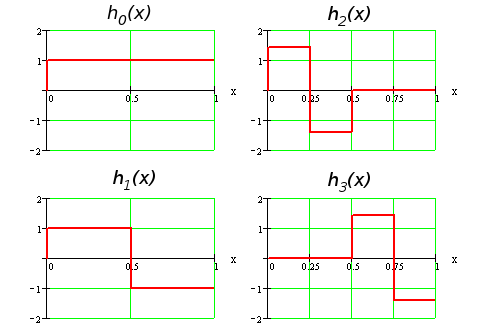
\includegraphics[width=0.95\textwidth]{../Graphics/Lectures-5-Haar_functions.png}
					\caption{Графики некоторых функций Хаара.}
				\end{subfigure}
			\end{figure}
	
			И так далее, образуя последовательность ортогональных ступенчатых функций. Любая функция, являющаяся ступенчатой, может
			быть задана через линейную последовательность функций $h_0, \dots, h_n, \dots$.

\end{document}
